\documentclass[letterpaper]{article}
\usepackage[submission]{aaai2027}
\usepackage[hyphens]{url}
\usepackage{graphicx}
\urlstyle{rm}
\def\UrlFont{\rm}
\usepackage{natbib}
\usepackage{caption}
\frenchspacing
\usepackage{amsmath}
\usepackage{booktabs}
\usepackage{enumitem}
\usepackage{microtype}
\usepackage{tabularx}
\usepackage{xcolor}
\usepackage{tikz}
\usepackage{xspace}
\usetikzlibrary{arrows.meta,fit,positioning,shapes.geometric}

\pdfinfo{
/TemplateVersion (2027.1)
}

\newcommand{\system}{\textsc{Agent Nebula}\xspace}
\newcommand{\artifact}[1]{\texttt{#1}}
\newcommand{\resulttodo}[1]{\textcolor{red}{[Result pending: #1]}}

\title{Are Long-Running Agents Making Progress?\\
A Longitudinal Study of Artifact Evolution, Rework, and Continuity}
\author{Anonymous Submission}
\affiliations{}

\begin{document}
\maketitle

\begin{abstract}
Long-running agents can modify a workspace for days across many context resets.
When they stop, action counts, commits, and final artifacts do not reveal
whether activity accumulated into durable and validated progress or repeatedly
overwrote, abandoned, and rediscovered the same work.  Existing trajectory
studies characterize actions within benchmark attempts, while studies of
long-lived agents focus on task outcomes or internal memory degradation.  We
instead make the persistent workspace the longitudinal unit of analysis.
We introduce a source-linked projection that connects native Claude, Codex, and
Gemini actions to stable artifact identities, lifecycle effects, event time,
and session boundaries without introducing semantic labels or aligning the
timeline to Git commits.  We use it to study six real software and autonomous-
research projects through artifact durability, later reuse, validation
association, rework, attention migration, and cross-session re-grounding.  A
separate measurement experiment compares source-verifiable fact coverage with
Final State, aggregate Counts, the official ProcGrep action representation, and
a bounded raw-log language-model reader.  \resulttodo{corpus coverage, central
empirical findings, and measurement-comparison results.}
\end{abstract}

\section{Introduction}

An increasingly common workflow gives an agent a broad idea, leaves it to work
inside one repository for two or three days, and inspects the result later.
The returned workspace may contain hundreds of tool calls, dozens of commits,
and substantial code, prose, tests, and experimental output.  This volume
looks productive but does not answer the question the user actually has:
\emph{did the work converge into durable, validated progress?}

Final state and commit history are necessary but lossy views of that question.
They omit reads, failed validations, transient artifacts, overwritten attempts,
and the cost of re-establishing context after a session boundary.  Aggregate
counts retain activity volume but erase which artifacts actions concerned and
whether later work reused or replaced them.  A raw log retains detail, yet its
session-local linear order does not directly expose a workspace lineage that
continues after one context disappears.  Context management can rapidly weaken
earlier plans~\cite{mehta2026plans}, and reliability can change over long chains
of sessions~\cite{zhu2026aging}.

Fine-grained trajectory analysis is not new.  Prior work mines action
sequences and repeated behaviors in software-engineering agents
~\cite{bouzenia2025trajectories}, measures validation and context-gathering
behavior under task and model confounds~\cite{mehtiyev2026behavioral}, and
shows that agents may reach a correct intermediate state and later overwrite
it~\cite{kim2026trajeval}.  ProcGrep represents trajectories as action
procedures and supports deterministic pattern queries and behavioral
fingerprints~\cite{oderinwale2026procgrep}.  Persistent file workspaces and
multi-session tasks are also established system mechanisms and settings
~\cite{zhou2026orspace}.  These results rule out generic claims about first
trajectory analysis, edit loops, validation gaps, fingerprints, or persistent
workspaces.

The remaining gap is longitudinal and artifact centered.  A benchmark attempt
usually ends when one patch is scored; a persistent project continues while
code, papers, datasets, results, and documentation acquire histories of their
own.  We ask how action volume relates to three observable dimensions:
\emph{durability}, whether an artifact persists; \emph{reuse}, whether later
work returns to it; and \emph{validation association}, whether a later
successful validation follows its mutation.  We keep these dimensions
separate instead of combining them with arbitrary weights.  Their conjunction
is useful shorthand for durable, reused, and validation-associated artifact
progress, not a scalar quality score.

We build this study directly on native Agent records.  The existing
\artifact{agent-session} adapters parse Claude, Codex, and Gemini.  A thin
repository projection retains all admitted Tool actions, resolves qualified
file effects, preserves explicit rename lineage and session identity, and
orders events by Agent action time.  Git contributes final tracked state and
optional content-survival evidence, but commits never define the time axis.
The same facts drive both quantitative analyses and the auxiliary \system
replay; visual layout is not a statistical measurement.

This paper makes three contributions:

\begin{enumerate}[leftmargin=*,itemsep=2pt]
  \item a longitudinal empirical characterization of how Agent activity,
  artifact persistence, reuse, validation, rework, attention, and session
  continuity interact across six real coding and autonomous-research projects;
  \item a deterministic, source-linked measurement method that preserves
  stable artifact identity and cross-session lineage without another general
  event IR or generated semantic gold; and
  \item a fact-level evaluation that isolates the incremental measurement
  coverage of artifact and session relations from Final State, Counts,
  ProcGrep's action-only procedures, and a bounded raw-log model reader.
\end{enumerate}

\section{Problem Setting}
\label{sec:problem}

\subsection{Persistent Work Rather Than Isolated Sessions}

Let a workspace $W$ persist while sessions $S=(s_1,\ldots,s_m)$ execute native
Tool actions $A=(a_1,\ldots,a_n)$.  Each action may read, create, mutate,
rename, or delete zero or more artifacts.  Sessions partition model context;
they do not reset $W$ or terminate an artifact's history.  Our unit of analysis
is one repository lineage over the complete observation interval, with
project-level cases kept separate.

Action time is ordered by native timestamp and stable source identifier.  A
commit can occur between actions and can anchor a final-state query, but it
does not replace the action order.  This distinction is important because an
agent can explore, fail, create temporary files, and revert changes before any
commit.

\subsection{Observable Progress Without Semantic Gold}

We do not infer intent, failure cause, reflection, or waste from file motion.
Instead, we measure source-verifiable process facts:

\begin{itemize}[leftmargin=*,itemsep=2pt]
  \item \textbf{Durability}: final artifact existence or tracked state and,
  where independent diff or snapshot evidence permits, content survival;
  \item \textbf{Reuse}: a later source-linked access to the same artifact
  lineage and its event, time, and session distance; and
  \item \textbf{Validation association}: distance from mutation to the next
  source-native successful test, check, build, or experiment action.
\end{itemize}

A successful validation proves that validation occurred, not that it covered a
particular mutation.  A file that is never revisited is an observed orphaned
artifact, not automatically useless.  Repeated tests or edits are process
patterns, not automatically waste.  Skill and harness analyses therefore
report temporal association, never causality, in the observational corpus.

Figure~\ref{fig:process-measures} makes the measurement relationships explicit.
The study follows Agent action time through session boundaries, keeps artifact
histories distinct, and measures survival, later reuse, validation distance,
and observable re-grounding.  The figure is a definition schematic rather than
an empirical result; the corresponding result plots are generated from the
six-project source rows in Section~\ref{sec:evaluation}.

\begin{figure*}[t]
\centering
\resizebox{0.96\textwidth}{!}{%
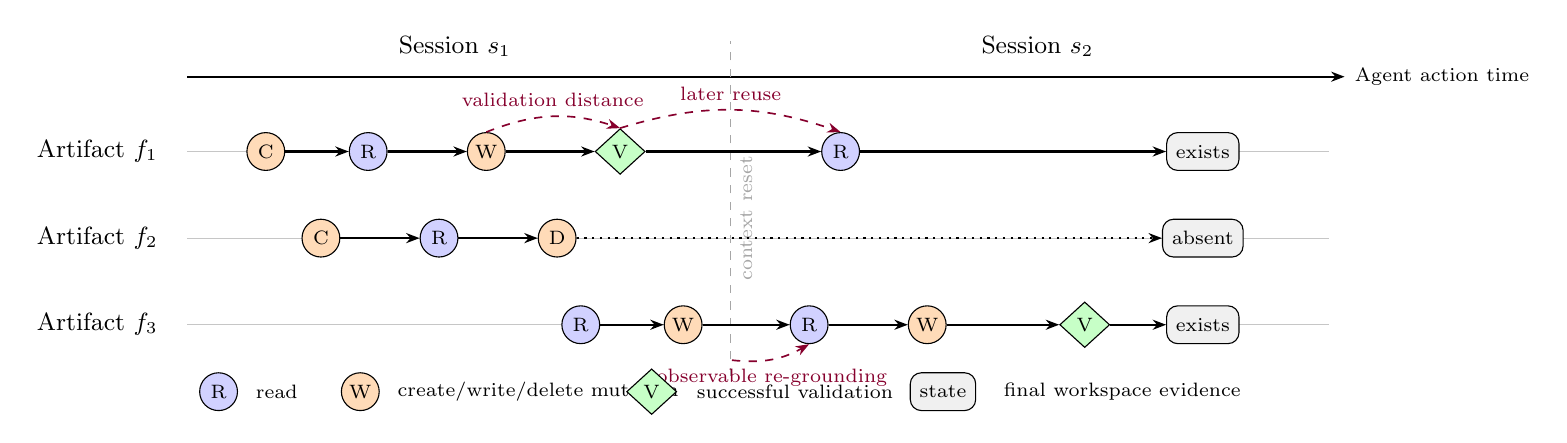
\begin{tikzpicture}[
  x=1cm,y=1cm,
  event/.style={draw,circle,minimum size=0.48cm,font=\scriptsize,inner sep=0pt},
  read/.style={event,fill=blue!18},
  mutate/.style={event,fill=orange!28},
  validate/.style={draw,diamond,aspect=1.5,minimum size=0.58cm,
                   font=\scriptsize,fill=green!22,inner sep=1pt},
  state/.style={draw,rounded corners,minimum height=0.48cm,
                font=\scriptsize,fill=gray!12},
  flow/.style={-{Stealth[length=1.7mm]},thick},
  measure/.style={-{Stealth[length=1.7mm]},dashed,semithick,purple!70!black}
]
\draw[flow] (0.8,3.8) -- (15.5,3.8) node[right,font=\scriptsize] {Agent action time};
\draw[dashed,gray!70] (7.7,0.0) -- (7.7,4.25);
\node[font=\small] at (4.2,4.18) {Session $s_1$};
\node[font=\small] at (11.6,4.18) {Session $s_2$};
\node[font=\scriptsize,rotate=90,gray!70] at (7.9,2.0) {context reset};

\node[font=\small,anchor=east] at (0.55,2.85) {Artifact $f_1$};
\node[font=\small,anchor=east] at (0.55,1.75) {Artifact $f_2$};
\node[font=\small,anchor=east] at (0.55,0.65) {Artifact $f_3$};
\draw[gray!45] (0.8,2.85) -- (15.3,2.85);
\draw[gray!45] (0.8,1.75) -- (15.3,1.75);
\draw[gray!45] (0.8,0.65) -- (15.3,0.65);

\node[mutate] (c1) at (1.8,2.85) {C};
\node[read] (r1) at (3.1,2.85) {R};
\node[mutate] (w1) at (4.6,2.85) {W};
\node[validate] (v1) at (6.3,2.85) {V};
\node[read] (r2) at (9.1,2.85) {R};
\node[state] (p1) at (13.7,2.85) {exists};
\draw[flow] (c1) -- (r1);
\draw[flow] (r1) -- (w1);
\draw[flow] (w1) -- (v1);
\draw[flow] (v1) -- (r2);
\draw[flow] (r2) -- (p1);

\node[mutate] (c2) at (2.5,1.75) {C};
\node[read] (r3) at (4.0,1.75) {R};
\node[mutate] (d2) at (5.5,1.75) {D};
\node[state] (p2) at (13.7,1.75) {absent};
\draw[flow] (c2) -- (r3);
\draw[flow] (r3) -- (d2);
\draw[flow,dotted] (d2) -- (p2);

\node[read] (r4) at (5.8,0.65) {R};
\node[mutate] (w3) at (7.1,0.65) {W};
\node[read] (rg) at (8.7,0.65) {R};
\node[mutate] (w4) at (10.2,0.65) {W};
\node[validate] (v2) at (12.2,0.65) {V};
\node[state] (p3) at (13.7,0.65) {exists};
\draw[flow] (r4) -- (w3);
\draw[flow] (w3) -- (rg);
\draw[flow] (rg) -- (w4);
\draw[flow] (w4) -- (v2);
\draw[flow] (v2) -- (p3);

\draw[measure] (w1.north) to[bend left=20]
  node[above,font=\scriptsize] {validation distance} (v1.north);
\draw[measure] (v1.north) to[bend left=18]
  node[above,font=\scriptsize] {later reuse} (r2.north);
\draw[measure] (7.72,0.2) to[bend right=18]
  node[below,font=\scriptsize] {observable re-grounding} (rg.south);

\node[read] at (1.2,-0.2) {R};
\node[font=\scriptsize,anchor=west] at (1.55,-0.2) {read};
\node[mutate] at (3.0,-0.2) {W};
\node[font=\scriptsize,anchor=west] at (3.35,-0.2) {create/write/delete mutation};
\node[validate] at (6.7,-0.2) {V};
\node[font=\scriptsize,anchor=west] at (7.15,-0.2) {successful validation};
\node[state] at (10.4,-0.2) {state};
\node[font=\scriptsize,anchor=west] at (11.05,-0.2) {final workspace evidence};
\end{tikzpicture}}
\caption{Measurement schematic for persistent workspace evolution.  Circles
are source-linked reads (R) and mutations (C/W/D); diamonds are successful
validations (V); terminal boxes are independently observed final workspace
state.  Artifact $f_1$ is mutated, validated, reused after a session reset, and
survives; $f_2$ is created and later deleted; $f_3$ illustrates observable
re-grounding before continued mutation.  The study reports these dimensions
separately and never treats the schematic as empirical data.}
\label{fig:process-measures}
\end{figure*}

\section{Workspace-Centered Measurement}
\label{sec:method}

\subsection{Source Selection and Projection}

We admit a complete native session when its project directory, working
directory or worktree root, or Git remote identifies the target repository.
All Tool actions in an admitted session remain on the timeline, including
searches, shell commands, failed validations, and calls without a resolved
file path.  A global path scan is reported separately because matching only
repository-related lines loses the surrounding no-file actions.

For each admitted action, the projection retains

\begin{equation}
a_i=(t_i,id_i,s_i,v_i,u_i,e_i,q_i),
\end{equation}

where $t_i$ is native time, $id_i$ the stable source ID, $s_i$ the session,
$v_i$ the vendor, $u_i$ the Tool/category, $e_i$ the source-native command
effect, and $q_i$ the reported status.  It attaches zero or more effects

\begin{equation}
\begin{aligned}
E_i &= \{(f,o,f')\},\\
o &\in \{\textsf{read},\textsf{write},\textsf{create},\\
  &\qquad \textsf{rename},\textsf{delete}\}.
\end{aligned}
\end{equation}

Here $f$ is a repository-relative artifact and $f'$ is populated only by an
observed rename.  Failed calls remain actions but emit no successful effect.
Directory arguments are weak scope evidence rather than fabricated reads of
every descendant.  Unknown paths, effects, and status remain explicit coverage
gaps.

\begin{figure}[t]
\centering
\resizebox{0.9\columnwidth}{!}{%
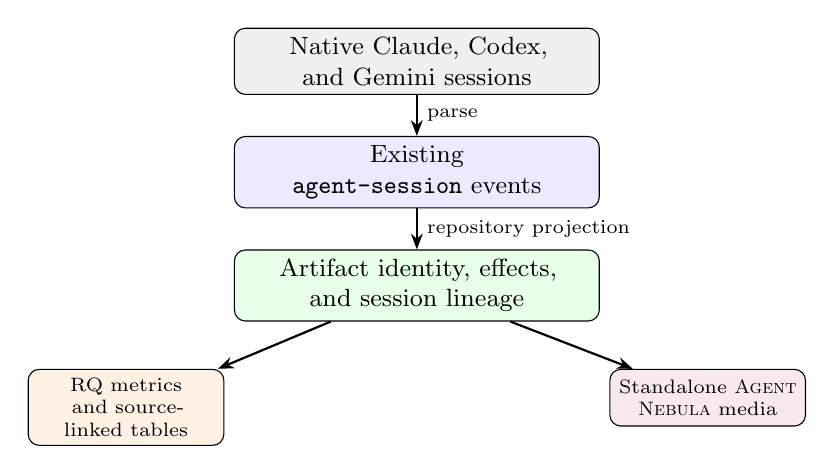
\begin{tikzpicture}[
  box/.style={draw,rounded corners,align=center,minimum height=0.72cm,
              text width=4.4cm,font=\small},
  output/.style={draw,rounded corners,align=center,minimum height=0.72cm,
                 text width=2.25cm,font=\scriptsize},
  flow/.style={-{Stealth[length=2mm]},thick},
  node distance=0.52cm
]
\node[box,fill=gray!12] (native) {Native Claude, Codex, and Gemini sessions};
\node[box,fill=blue!8,below=of native] (parser) {Existing \artifact{agent-session} events};
\node[box,fill=green!9,below=of parser] (projection) {Artifact identity, effects, and session lineage};
\node[output,fill=orange!10,below left=0.6cm and 0.12cm of projection]
  (metrics) {RQ metrics and source-linked tables};
\node[output,fill=purple!9,below right=0.6cm and 0.12cm of projection]
  (media) {Standalone \system media};
\draw[flow] (native) -- node[right,font=\scriptsize] {parse} (parser);
\draw[flow] (parser) -- node[right,font=\scriptsize] {repository projection} (projection);
\draw[flow] (projection) -- (metrics);
\draw[flow] (projection) -- (media);
\end{tikzpicture}}
\caption{One source projection supports measurement and visualization.  The
empirical analyses consume structured events, not visual coordinates.}
\label{fig:architecture}
\end{figure}

\subsection{Artifact and Validation Derivations}

An explicit rename preserves artifact identity.  Delete followed by create at
the same path begins a new identity unless the source connects them.  For each
mutation, we locate the next later access to that identity and the next
successful validation globally and within the same session.  We report both
event and wall-clock distance.  Final existence and tracked state are queried
from the workspace and Git independently of the event ordering.

We report complete survival and distance curves or declared sensitivity ranges;
no fixed 24-event attention window enters the research measurement.  Visual
attention decay and force layout remain presentation-only choices.

\subsection{Fact-Level Tool Comparison}

The tool experiment stratifies questions into action-only, artifact-linked,
cross-session, and final-state facts.  Every answer must cite source IDs or
abstain.  Truth is generated independently from native records and
workspace/Git state; no method under comparison labels its own answer.

Final State and Counts are lower-information controls.  ProcGrep is the
strongest action-only procedure baseline and should tie or win action-only
questions.  The bounded raw-log model receives the same source membership and
fixed retrieval, context, and output budgets.  The proposed method can support
only an incremental-coverage claim for artifact-linked and cross-session facts
at comparable factual accuracy and reported cost.

\section{Implementation}
\label{sec:implementation}

The implementation is a Rust extension of the existing \artifact{agentvis}
repository projection.  It reuses \artifact{agent-session} for native parsing,
affiliates sessions with all repository worktrees, normalizes paths, and emits
ordinary source-linked JSON and CSV rows.  The analysis computes project-level
coverage, artifact and mutation rows, and RQ summaries without a frontend,
database, generated semantic layer, or additional runtime dependency.

The product path continues to export one standalone HTML, SVG, PNG, GIF, or MP4
per visualization.  Layout is computed once and media outputs share the same
frame stream.  These outputs provide case evidence navigation and reproducible
examples; the empirical measurements are recomputed from structured rows.

\section{Empirical Study}
\label{sec:evaluation}

\subsection{Research Questions}

\paragraph{RQ1---Activity to artifact progress.}
How much long-running Agent activity becomes artifact change that persists,
is later reused, and is followed by successful validation?

\paragraph{RQ2---Validation dynamics.}
How do successful and failed validations interleave with mutation bursts and
unvalidated backlog across artifact types?

\paragraph{RQ3---Rework and convergence.}
How do repeated mutation, validation-followed revision, delete/replace, and
module switching characterize rework and non-convergence?

\paragraph{RQ4---Cross-session continuity.}
How much observable re-grounding precedes a new session's first mutation, and
how often does work continue the previous session's artifacts and modules?

\paragraph{RQ5---Attention allocation.}
How does Agent attention migrate among code, tests, configuration, papers and
documentation, data, results, and workspace modules?

\paragraph{RQ6---Skill and harness association.}
What process patterns follow source-visible skill, harness, model, and task
configuration, and how heterogeneous are those associations across cases?

\paragraph{RQ7---Measurement capability.}
Which source-verifiable facts does the artifact-linked representation recover
beyond Final State, Counts, ProcGrep, and bounded raw-log model analysis, and
at what accuracy and cost?

\subsection{Cases and Inclusion}

We fix six local open-source repositories before computing process rates.
They cover systems software, mixed documentation and code, autonomous research,
and skill/harness development.

\begin{table}[t]
\centering
\small
\begin{tabular}{@{}ll@{}}
\toprule
Repository & Dominant work type \\
\midrule
AgentSight & systems software and research \\
ActPlane & systems software and research \\
bpf-developer-tutorial & tutorial, code, documentation \\
eunomia.dev & content, documentation, software \\
agentskill-observability-paper & paper, experiment, code \\
academic-writing-skills & skills, prompts, tests, documents \\
\bottomrule
\end{tabular}
\caption{Fixed first-study cases.  Each project remains one case; its sessions
are not treated as independent projects.}
\label{tab:cases}
\end{table}

The main corpus includes all repository-direct Claude, Codex, and Gemini
sessions and retains actions with no file effect.  We report source coverage by
project, vendor, session, effect, status, and path presence.  Global path-only
matches form a separate sensitivity analysis.  \resulttodo{qualified session,
action, effect, and observation-window counts for all six projects.}

\subsection{Analysis Protocol}

Each project is first analyzed as a complete case.  Cross-case summaries state
their project weighting and do not treat actions as independent samples.
Primary outputs are effect sizes, distributions, cumulative/survival curves,
and uncertainty.  Bootstrap or permutation uses session or project blocks only
when exchangeability is defensible.  Missing source fields remain coverage
results rather than imputed events.

Artifact type is an inspectable path/extension classification with an unknown
class.  Top-level directories provide the default module unit.  Model-derived
motifs, embeddings, clusters, or summaries are exploratory secondary analyses
and must resolve to source IDs and deterministic metrics.

\subsection{RQ1: Activity to Artifact Progress}

RQ1 reports action and mutation volume, final existence and tracked state,
later reuse distance, mutation-to-successful-validation distance, and the
intersection of observable durability, reuse, and validation association.
File-level survival remains separate from content-level survival.  The latter
is reported only where native diffs, snapshots, or Git line evidence establish
it independently.  \resulttodo{per-project RQ1 distributions, survival curves,
cross-case contrasts, and answer.}

\subsection{RQ2: Validation Dynamics}

RQ2 measures mutation bursts, successful and failed validation cadence,
unvalidated mutation backlog, and behavior immediately before and after
validation.  It never calls a successful command proof that every preceding
change was correct.  \resulttodo{RQ2 tables, curves, and answer.}

\subsection{RQ3: Rework and Convergence}

RQ3 reports repeated mutation per artifact, read--write--validate sequences,
validation-followed rework, delete/replace events, and module switching.  We
report distributions and sensitivity ranges rather than one ``thrashing''
threshold.  \resulttodo{RQ3 distributions, sensitivity analysis, and answer.}

\subsection{RQ4: Cross-Session Continuity}

RQ4 aligns every eligible native session boundary and measures actions before
the first mutation, overlap with the preceding session's active artifacts and
modules, and cross-session rework.  We call this observable cost a session
reset tax without making a claim about hidden model memory.  \resulttodo{RQ4
boundary-aligned results and answer.}

\subsection{RQ5: Attention Allocation}

RQ5 reports action allocation by artifact type, module transition matrices,
transition entropy, hotspot migration, and persistent cold regions in action
time.  Visual coordinates are excluded from statistics.  \resulttodo{RQ5
allocation and migration results and answer.}

\subsection{RQ6: Skill and Harness Association}

RQ6 first audits whether skill and configuration events are explicit enough to
observe.  It then compares subsequent artifact mix, validation cadence,
rework, and survival within cases.  Task, model, time, and project confounds
prevent causal attribution.  \resulttodo{RQ6 source coverage, associations,
heterogeneity, and answer.}

\subsection{RQ7: Measurement Capability}

RQ7 uses a fixed, stratified fact set and the same source universe for every
method.  It reports fact accuracy, answer coverage, evidence precision,
abstention, tokens, bytes, and latency.  Action-only questions are positive
controls for ProcGrep; final-state questions are positive controls for Final
State.  Artifact-linked and cross-session questions isolate the proposed
increment.  \resulttodo{fact-set size, baseline versions, accuracy/coverage/
cost table, and answer.}

\section{Threats to Validity}

Native Agent records can omit implicit subprocess effects, external editor
changes, or actions performed outside instrumented tools.  The study reports
adapter and field coverage, and it does not convert missing effects into
no-effect observations.  Optional system-level AgentSight evidence is a future
coverage extension, not a second logic layer in the present analysis.

Final workspace state cannot prove content-level survival of every historical
edit.  We therefore separate file existence, Git-tracked state, and independently
supported content survival.  Successful validation is association rather than
coverage or correctness evidence.

The six cases are selected from local author-associated projects.  They provide
deep, source-native longitudinal evidence but cannot establish population-wide
rates.  Broad AAAI claims require an independent public or prospectively
captured corpus after this study identifies measurements with adequate source
coverage.

Skill, harness, model, task, and project often change together.  RQ6 is
observational and generates controlled hypotheses; it does not identify causal
effects.  Likewise, repeated actions, unvisited artifacts, and long validation
gaps are process facts rather than automatic failure labels.

\section{Related Work}

\paragraph{Agent trajectory studies.}
Software-engineering trajectory studies analyze action sequences, reasoning,
testing, and strategy~\cite{bouzenia2025trajectories,mehtiyev2026behavioral}.
TRAJEVAL identifies coherence collapse after reaching useful intermediate
code~\cite{kim2026trajeval}.  ProcGrep induces canonical action procedures and
behavioral fingerprints~\cite{oderinwale2026procgrep}.  We reuse these
action-level precedents and focus the novelty question on persistent artifact
identity and cross-session lineage.

\paragraph{Long-horizon and persistent work.}
AgingBench studies reliability across many sessions~\cite{zhu2026aging}, while
context-management work shows that plans can lose influence
~\cite{mehta2026plans}.  OR-Space evaluates persistent multi-artifact workspaces
~\cite{zhou2026orspace}.  These works motivate the setting but do not measure
artifact durability, reuse, validation association, and re-grounding across
real project histories.

\paragraph{Diagnosis and harness analysis.}
AgentDiagnose and AgentRx diagnose completed trajectories
~\cite{ou2025agentdiagnose,barke2026agentrx}; TrajAudit retrieves evidence from
repository traces~\cite{wang2026trajaudit}; and HarnessFix links failed
trajectories to harness mechanisms~\cite{chen2026harnessfix}.  We do not claim a
new diagnostic labeler or causal harness repair.  Our tool evaluation asks only
which process facts are measurable from source-linked artifact lineage.

\section{Ethical Considerations}

Native trajectories can contain private prompts, source code, paths, secrets,
and experimental data.  Local analysis does not imply permission to publish
raw sessions.  Released evidence must follow repository and data permissions,
remove credentials and personal content, and prefer aggregate or explicitly
approved source-linked examples.

Process measurements can be misused as productivity scores.  We therefore do
not rank people, treat activity volume as progress, or label an observed
pattern as waste without independent task evidence.  The intended consumer is
an Agent or automatic diagnostic process studying its own authorized workspace.

\section{Conclusion}

Long-running Agent work persists in artifacts while session context disappears.
Studying only final state, commits, or action volume therefore misses the
process users need to understand: whether work persists, is reused, receives
validation, converges, and survives context resets.  Our workspace-centered
measurement connects native actions to artifact identity and session lineage,
then separates empirical findings from the tool's incremental fact coverage.
\resulttodo{final evidence-backed answers to RQ1--RQ7 and their implications.}

\bibliography{references}

\end{document}
